\documentclass[14pt]{article}
\usepackage[letterpaper, margin=1in]{geometry}
\usepackage{amssymb}
\usepackage{amsmath}
\usepackage{graphicx}
\usepackage{algorithm}
\usepackage{algorithmicx}
\usepackage{enumitem}
\usepackage[noend]{algpseudocode}
        
\def\BState{\State\hskip-\ALG@thistlm}
        
\topmargin = -50pt
        
\title{HW 9}
\author{Yunhao Lin}
        
\begin{document}
\maketitle

\begin{enumerate}
\item In order to provide a counterexample for this greedy solution. Suppose we
have 6 rectangle shaped discs in order to placed on 2 pegs. Suppose we have
rectangles A:5 by 6, B: 4 by 5, C: 3 by 2, D: 2 by 1. Furthermore, we have 5 with
width greater than 5 and height greater than 3 but less than 6.
Let's say our E is a rectangle of 6 by 3. And one more rectangle 6 with width less
than 2, height larger than 1 but larger than 5. Let's say our F is a rectangle
of 1 by 4. Our list D = $\{A,B,C,D,E,F\}$.
And therefore it has a matrix C as follows where A is 1, B is 2 and follows:
\[
\begin{bmatrix}
    0 & 0 & 0 & 0 & 0 & 0\\
    0 & 1 & 0 & 0 & 0 & 0\\
    1 & 1 & 0 & 0 & 1 & 0\\
    1 & 1 & 1 & 0 & 1 & 0\\
    0 & 0 & 0 & 0 & 0 & 0\\
    1 & 1 & 0 & 0 & 0 & 0\\
\end{bmatrix}\]
 It can be put in 2 pegs as follows, starting left is the disc on the bottom.
 \[
    pegs  \left\{
                \begin{array}{ll}
                    \ E:\;6*3 \Leftarrow C:\;3*2 \Leftarrow D:\;2*1 \\
                    \ A:\;5*6 \Leftarrow B:\;4*5 \Leftarrow F:\;1*4
                \end{array}
              \right.
    \]
But using the greed algorithm, it would find the largest number of discs that 
can be put on one peg and then remove these disces. As observed from above, which
is quite previous. The discs A,B,C,D can be put on the same peg, with A on the bottom,
followed by B, then C and then D. Which results in  on peg as follow. 
\[
    pegs  \left\{
                \begin{array}{ll}
                    \ A:\;5*6 \Leftarrow B:\;4*5 \Leftarrow C:\;3*2 \Leftarrow D:\;2*1 
                    \   
                \end{array}
              \right.
    \]
But we still have E and F left in the list D. And notice that E is 6*3 but F is
1*4, therefore obviously E and F cannot be put on the same peg. And we need three
pegs to put all the disks, but we were only given 2. The final peg would be as 
follows, which gives us the wrong result:
\[
    pegs  \left\{
        \begin{array}{ll}
        \ A:\;5*6 \Leftarrow B:\;4*5 \Leftarrow C:\;3*2 \Leftarrow D:\;2*1 \\
        \ E:\;6*3\\
        \ F:\;1*4     
        \end{array}
    \right.
\]
\\\\\\\\\\\\\\\\\\\\\\\\
\item 
\begin{figure}
    \centering
    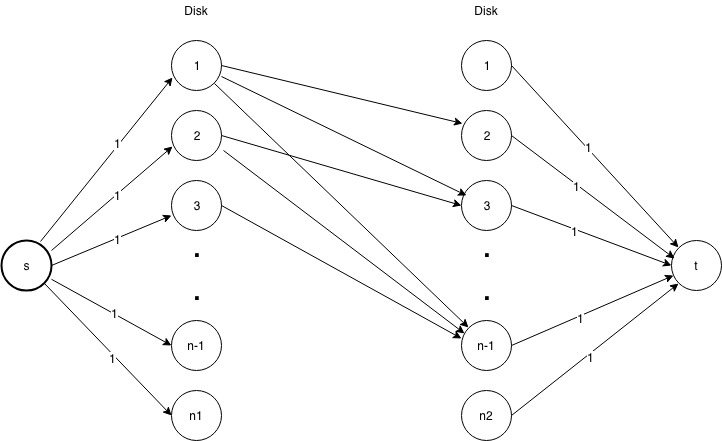
\includegraphics[width =150mm]{hello.jpg} \\
\end{figure}
Construct G' on $[n1]\cup[n2]$ by adding following edges $(n_1 = n, n_2 = n)$:
\begin{itemize}
    \item An edge from $s$ to $i$, $\forall i \in [n_1]$ with capacity 1.
    \item An edge from $j$ to $t$, $\forall j \in [n_2]$ with capacity 1.
    \item For any edge from $\alpha$ to $\beta$, $\forall \alpha \in [n_1]$ and
    $\forall \beta \in [n_2]$ whenever $\alpha$ can be put on top of $\beta$ with
    capacity 1.
\end{itemize}
Next we need to find the maximum flow from this network. Let $M$ denotes the 
maximum flow in this network. Check the number of $M$, if it is larger or equal
to $n-k$, $M \geq n-k$ then it is feasible to fit $n$ discs on $k$ segs. 
If $M$ is less than $n-k$ then it is not feasible to fit $n$ discs on $k$ segs.\\
\textbf{Proof of Correctness:} Suppose that we first have $n$ number of discs that
are sperated on $n$ segs at the beginning. Whenever we find an edge in from $n_1$
to $n_2$ then it means that this disk that was originally an seg itself can be 
combined by putting it on the other disk. Therefore the seg number is subtracted by
1 everytime we find a flow in the edge from $n_1$ to $n_2$. Therefore the maximum 
flow find the maximum number of edges from $n_1$ to $n_2$ that is possible to 
carry a flow which is $M$. Therefore the number of seg we need is then $n-M$, if 
$n-M \leq k$ then it means we can fit all the discs within this k segs. \\
\textbf{Time Complexity:} Since we need to draw n arrows on the left, n arrows on 
the right, which both taks $O(n)$ time. And at most $n^2$ arrows from $n_1$ to 
$n_2$. The time complexity to set up the graph is $O(n) +O(n)+ O(n^2) = O(n^2)$. And 
in order to find the maximum flow in this network and that would be done in $O(mn)$,
which in this case is just $O(n^2)$, and in the end it's just a comparison between
k and $n-M$ and this is O(1). So in general the time complexity is $ O(n^2)+O(n^2)+O(1)
= O(n^2)$.
\end{enumerate}



\end{document}